\documentclass[11pt,letterpaper,twoside]{article}
\usepackage[english]{babel}
\usepackage{amssymb,amsmath}
\usepackage{fancyhdr}
\usepackage{graphicx}

 \oddsidemargin  0in \evensidemargin 0in
 \topmargin   -0.25in \headheight 0.25in \headsep 0.25in
 \textwidth   6.5in \textheight 8.75in \marginparsep 0pt \marginparwidth 0pt
 \parskip 1ex  \parindent 0ex \footskip 20pt

\newfont{\bssten}{cmssbx10}
\newfont{\bssnine}{cmssbx10 scaled 900}

%%%%%%%%%%%%%%%%%%%%%%%
\newcommand{\whatizit}{Lecture 3: Data Collection and Sampling Strategies}
%%%%%%%%%%%%%%%%%%%%%%%


\pagestyle{fancy}  
\fancyhead{\bssnine STOR 155,  \whatizit}
\fancyhead[RE]{} \fancyhead[LO]{}
\fancyhead[LE]{\bssnine \thepage} \fancyhead[RO]{\bssnine \thepage}
\lfoot{} \cfoot{} \rfoot{}   


\newcommand{\var}{\mathrm{Var}}



\begin{document}



\thispagestyle{empty} \vspace*{-0.75in}

{\bssten STOR 155: Introduction to Data Models and Inference \hfill May 16, 2024 \\
Prof. Will Lassiter  \hfill Page 1 of \pageref{totalpag}}
\vspace{10pt}
\begin{center} {{\Large \bf \whatizit}} \end{center}

{\bf Sources of Data} \vspace{6pt}

Three common sources of data we'll discuss:

\begin{enumerate}

\item \quad \vspace{40pt}

\begin{center}
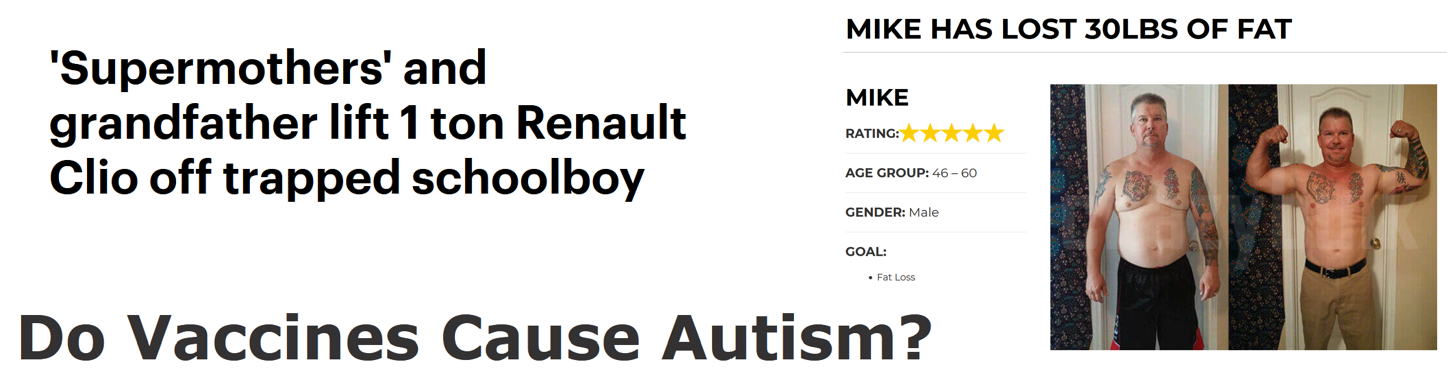
\includegraphics[scale=0.7]{images/anecdotal.png}
\end{center}

\item \quad \vspace{60pt}

\item \quad \vspace{60pt}

\end{enumerate}

Example: Does the health of a male cricket impact its ability to successfully find a mate? \vspace{100pt}

\newpage

{\bf Observational Studies vs.\ Experiments} \vspace{6pt}

Experiments have one {\bf major} advantage over observational studies: \vspace{120pt}


Observational studies cannot be used to establish causation due to... \vspace{120pt}


Example: Ice cream sales \vspace{150pt}

Example: ``Miracle drugs" and weight loss

\newpage

Example: A childcare study enrolled 1364 infants in 1991 and followed them through age 6. Researchers found the more time children spent in childcare from birth to 4{\footnotesize $\frac{1}{2}$},  the more adults tended to rate them as assertive, disobedient, and aggressive. \vspace{6pt}

Type of data collection? \vspace{30pt}

Explanatory and response variables? \vspace{30pt}

Possible lurking/confounding variables? \vspace{120pt}

An \_\_\_\_\_\_\_\_\_\_\_\_\_\_\_ was probably impossible here but, hypothetically, how might it have proceeded?

\newpage

{\bf Observational Studies: Terminology} \vspace{6pt}
\begin{enumerate}
\item {\bf Population}: \vspace{20pt}

\hspace{245pt}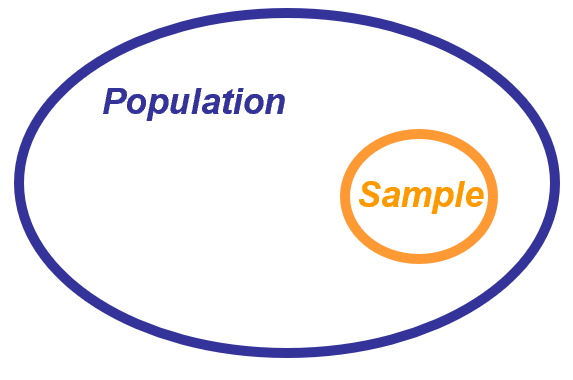
\includegraphics[scale=0.9]{images/pop.png}

\item {\bf Sample}: \vspace{150pt}

\end{enumerate}

Example: We want to know the distribution of student loan amounts for UNC undergraduates.
\begin{itemize}
\item What would a census look like? \vspace{100pt}

\item How about a sample survey?
\end{itemize}

\newpage

Census vs.\ sample survey: pros and cons \vspace{200pt}

Cooking metaphor:  \vspace{80pt}

For your inference to be valid, \vspace{80pt}

Example: Battery manufacturer \vspace{30pt}

Population of interest? \vspace{40pt}

How to choose the 24 batteries for inspection?

\newpage

{\bf Sampling Strategies for Observational Studies} \vspace{6pt}

Major pitfall: {\bf sampling bias}

\begin{center}
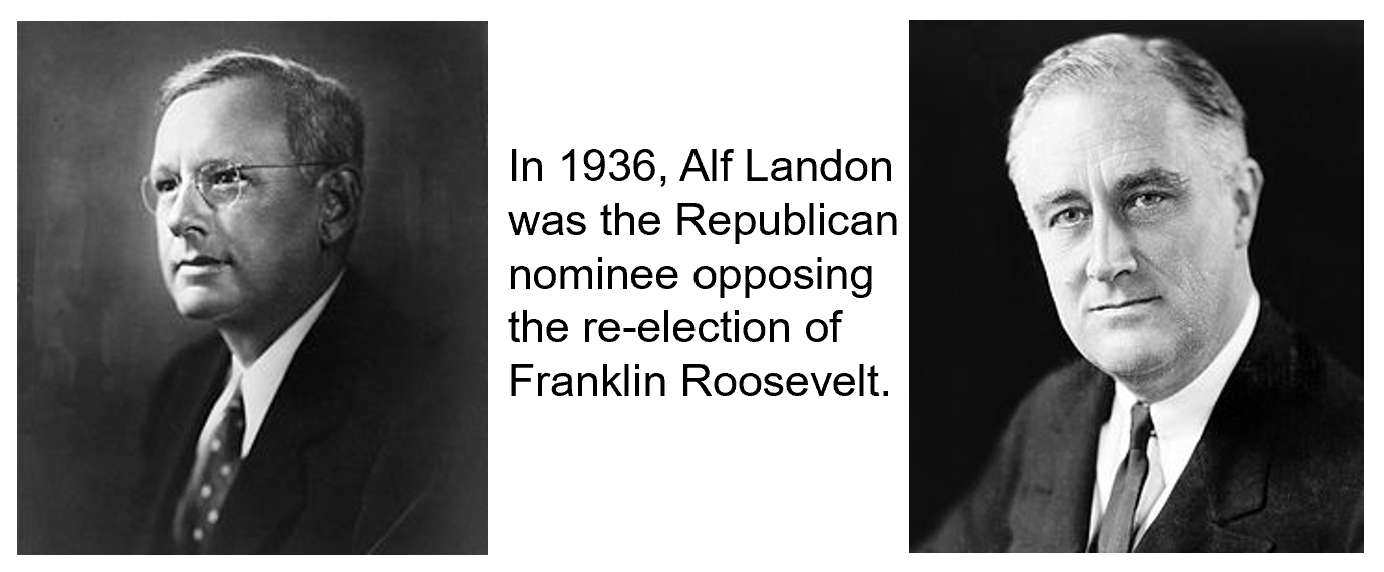
\includegraphics[scale=0.8]{images/fdr.png}

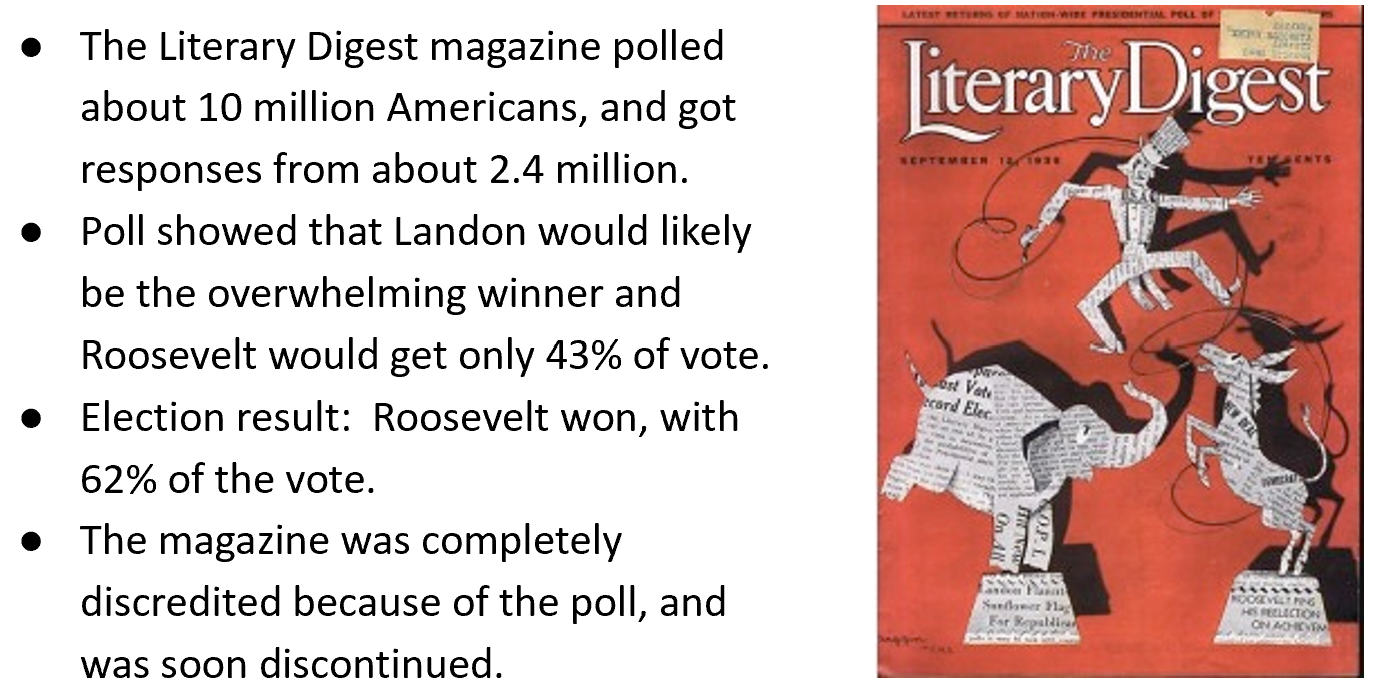
\includegraphics[scale=0.8]{images/fdr2.png}
\end{center}

What went wrong?

\newpage

Other possible sources of sampling bias: 

\begin{itemize}

\item {\bf Non-response} \vspace{60pt}

\item {\bf Voluntary response} \vspace{60pt}

\item {\bf Convenience} \vspace{60pt}

\end{itemize}

\begin{center}
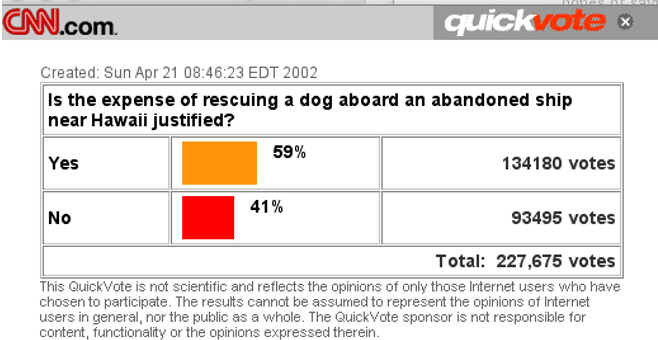
\includegraphics[scale=1.5]{images/cnn.png}
\end{center}

Arguably the most fundamental characteristic of good sampling techniques that seek to avoid bias is...

\newpage

``Good" sampling techniques:

\begin{itemize}

\item {\bf Simple Random Sample} \vspace{60pt}

\begin{center}
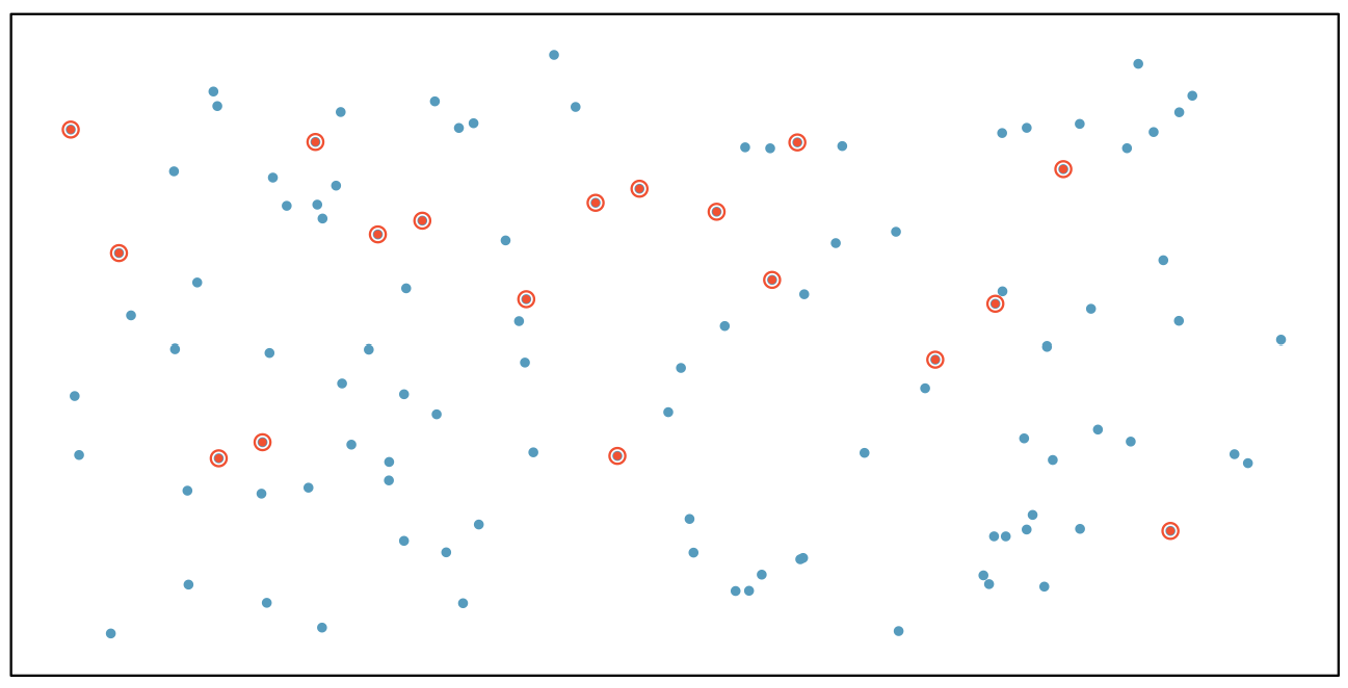
\includegraphics[scale=0.7]{images/srs.png}
\end{center}

\item {\bf Stratified Sampling} \vspace{90pt}

\begin{center}
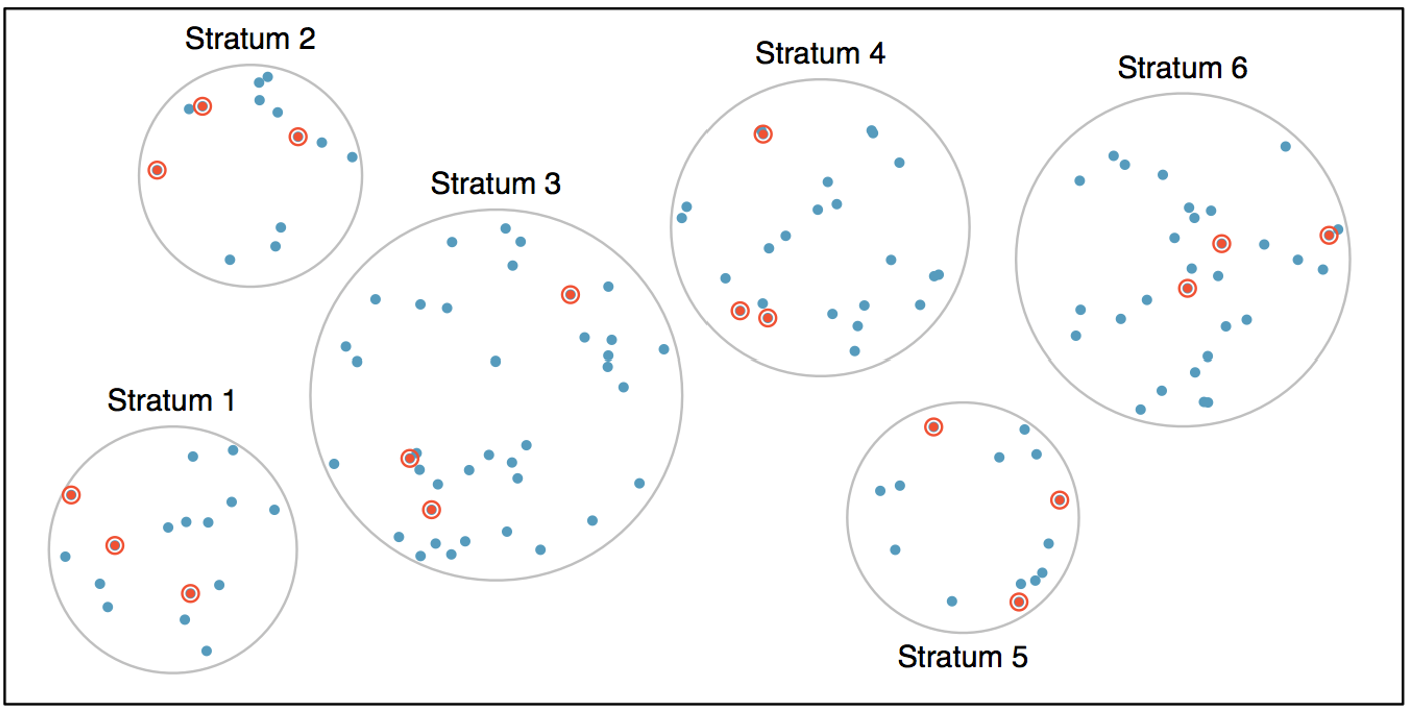
\includegraphics[scale=0.7]{images/stratified.png}
\end{center}

\newpage

\item {\bf Cluster Sampling} \vspace{90pt}

\begin{center}
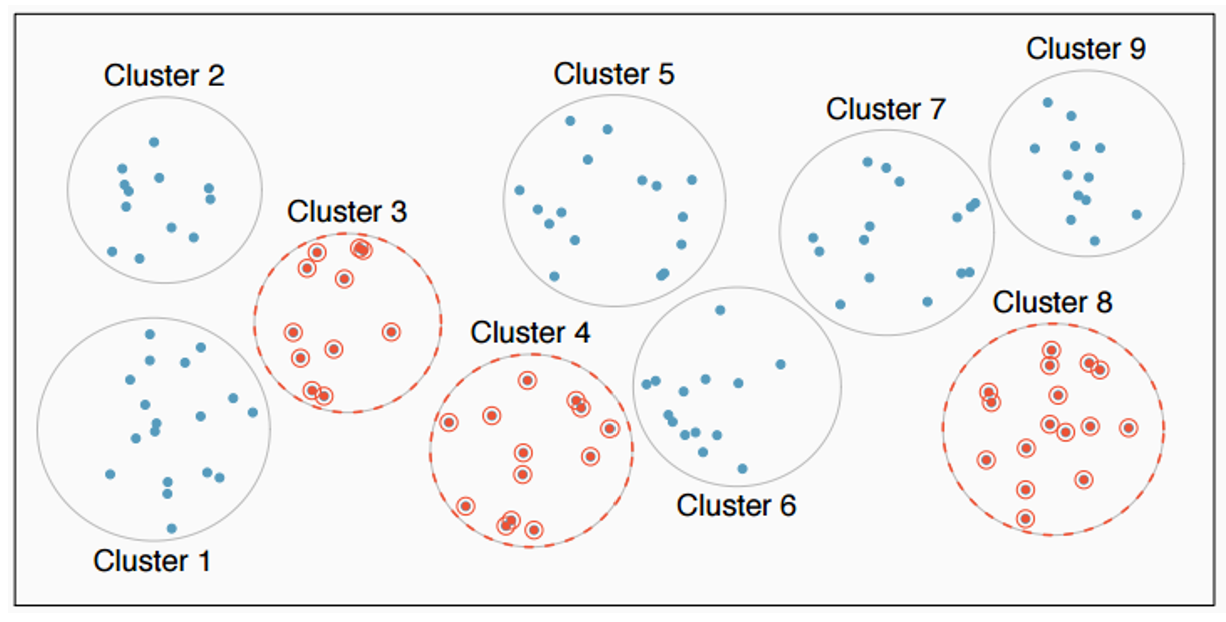
\includegraphics[scale=0.7]{images/cluster.png}
\end{center}

\item {\bf Multistage Sampling} \vspace{90pt}

\begin{center}
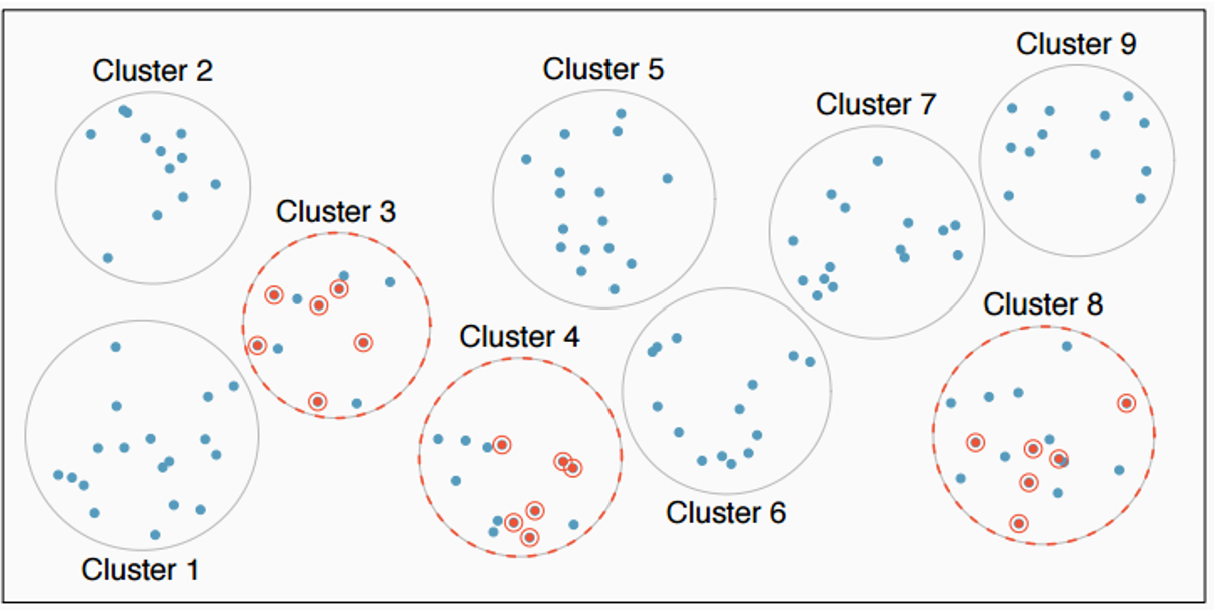
\includegraphics[scale=0.7]{images/multistage.png}
\end{center}

\end{itemize}

\newpage

Other factors that can bias/influence results:

\begin{itemize}

\item Wording of questions

\begin{center}
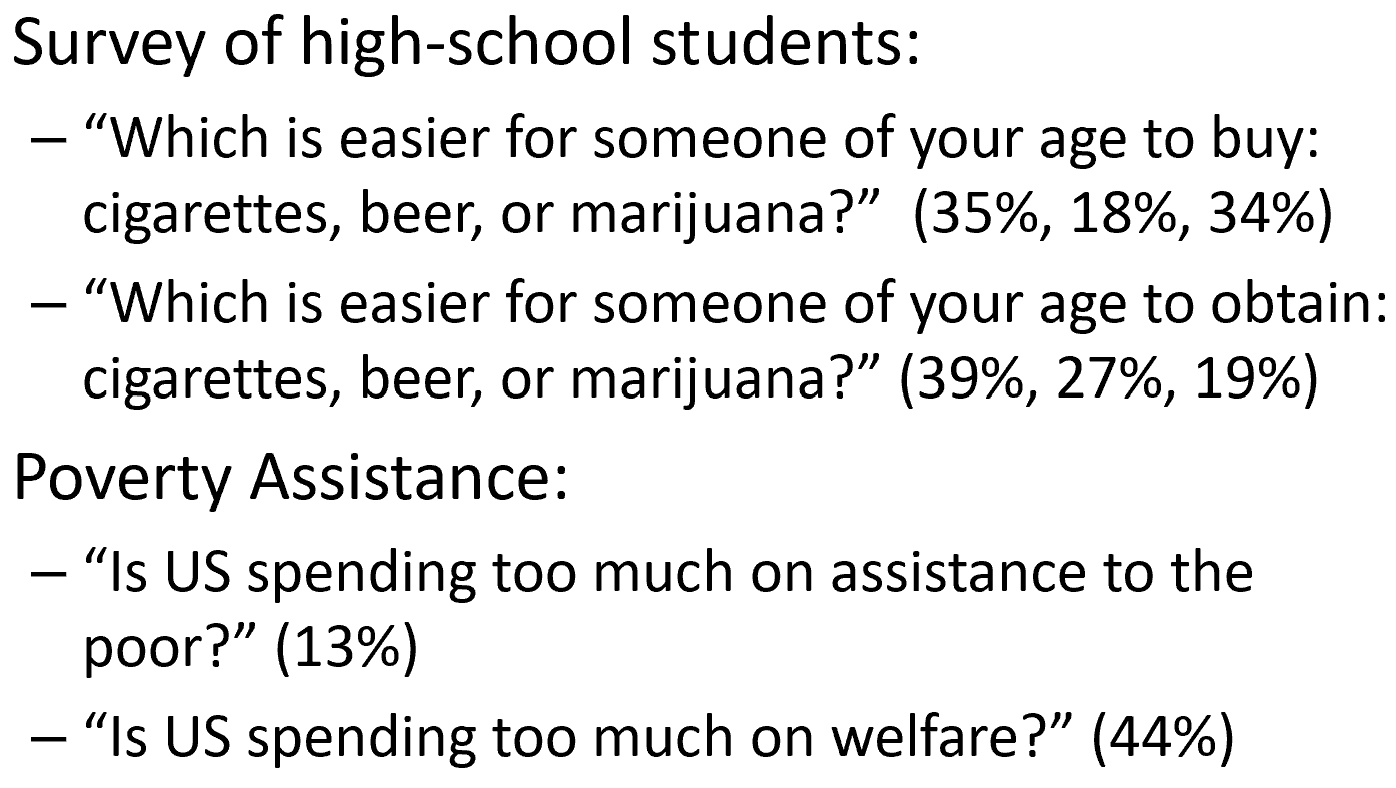
\includegraphics[scale=0.6]{images/wording.png}
\end{center}

\item Framing of questions

\begin{center}
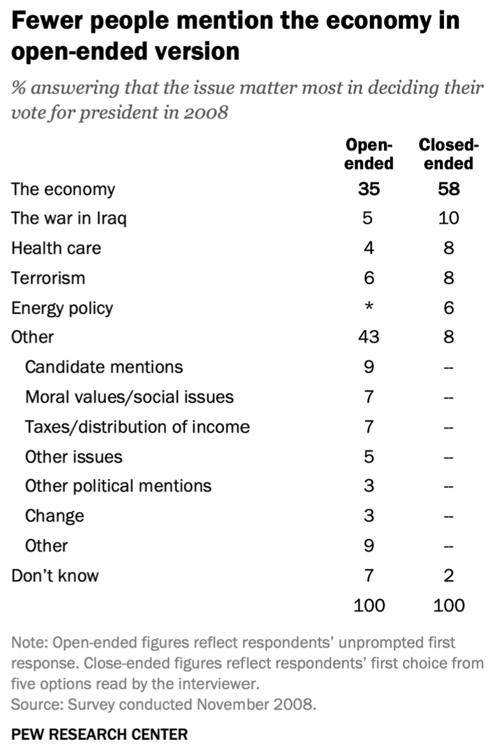
\includegraphics[scale=1.2]{images/framing.png}
\end{center}

\end{itemize}

\label{totalpag}
\end{document}